\documentclass[xelatex,aspectratio=169]{beamer}

\hfuzz=10pt
\vfuzz=10pt

% Theme
\usetheme{htw}
\setbeamertemplate{navigation symbols}{}
\setbeamertemplate{theorems}[numbered]
\setbeamercovered{transparent}

%\logo{
\includegraphics[height=0.5cm]{HTWD_color.png}}

% Packages
\usepackage{polyglossia}
\setmainlanguage{german}
\setotherlanguage{english}

\usepackage[bigfiles]{pdfbase}
\ExplSyntaxOn
\NewDocumentCommand\embedvideo{smm}{
\group_begin:
\leavevmode
\tl_if_exist:cTF{file_\file_mdfive_hash:n{#3}}{
  \tl_set_eq:Nc\video{file_\file_mdfive_hash:n{#3}}
}{
  \IfFileExists{#3}{}{\GenericError{}{File~`#3'~not~found}{}{}}
  \pbs_pdfobj:nnn{}{fstream}{{}{#3}}
  \pbs_pdfobj:nnn{}{dict}{
    /Type/Filespec/F~(#3)/UF~(#3)
    /EF~<</F~\pbs_pdflastobj:>>
  }
  \tl_set:Nx\video{\pbs_pdflastobj:}
  \tl_gset_eq:cN{file_\file_mdfive_hash:n{#3}}\video
}
%
\pbs_pdfobj:nnn{}{dict}{
  /Type/RichMediaInstance/Subtype/Video
  /Asset~\video
  /Params~<</FlashVars (
  source=#3&
  skin=SkinOverAllNoFullNoCaption.swf&
  skinAutoHide=true&
  skinBackgroundColor=0x5F5F5F&
  skinBackgroundAlpha=0.75
  )>>
}
%
\pbs_pdfobj:nnn{}{dict}{
/Type/RichMediaConfiguration/Subtype/Video
/Instances~[\pbs_pdflastobj:]
}
%
\pbs_pdfobj:nnn{}{dict}{
/Type/RichMediaContent
/Assets~<<
/Names~[(#3)~\video]
>>
/Configurations~[\pbs_pdflastobj:]
}
\tl_set:Nx\rmcontent{\pbs_pdflastobj:}
%
\pbs_pdfobj:nnn{}{dict}{
  /Activation~<<
  /Condition/\IfBooleanTF{#1}{PV}{XA}
  /Presentation~<</Style/Embedded>>
  >>
  /Deactivation~<</Condition/PI>>
}
%
\hbox_set:Nn\l_tmpa_box{#2}
\tl_set:Nx\l_box_wd_tl{\dim_use:N\box_wd:N\l_tmpa_box}
\tl_set:Nx\l_box_ht_tl{\dim_use:N\box_ht:N\l_tmpa_box}
\tl_set:Nx\l_box_dp_tl{\dim_use:N\box_dp:N\l_tmpa_box}
\pbs_pdfxform:nnnnn{1}{1}{}{}{\l_tmpa_box}
%
\pbs_pdfannot:nnnn{\l_box_wd_tl}{\l_box_ht_tl}{\l_box_dp_tl}{
  /Subtype/RichMedia
  /BS~<</W~0/S/S>>
  /Contents~(embedded~video~file:#3)
  /NM~(rma:#3)
  /AP~<</N~\pbs_pdflastxform:>>
  /RichMediaSettings~\pbs_pdflastobj:
  /RichMediaContent~\rmcontent
}
\phantom{#2}
\group_end:
}
\ExplSyntaxOff


\usepackage{graphicx}
\usepackage[export]{adjustbox}
\usepackage{animate}
%\usepackage[dvipdfmx]{movie15_dvipdfmx}
\usepackage{media9}
\usepackage{tabularx}
\usepackage{colortbl}
\usepackage{booktabs}
\usepackage{makecell}
\usepackage{ltablex}
\usepackage{array}
\usepackage{multirow}
\usepackage{amsmath}
\usepackage{amsthm}
%\renewcommand{\arraystretch}{1.5}
\newcolumntype{L}[1]{>{\raggedright\let\newline\\\arraybackslash\hspace{0pt}}p{#1}}
\newcolumntype{C}[1]{>{\centering\let\newline\\\arraybackslash\hspace{0pt}}p{#1}}
\newcolumntype{R}[1]{>{\raggedleft\let\newline\\\arraybackslash\hspace{0pt}}p{#1}}
%\renewcommand\thesatz{\arabic{section}.\arabic{theorem}}
\makeatletter
\@addtoreset{theorem}{lecture}
\makeatother

\newtheorem{satz}{Satz}[section]
\newtheorem{lem}{Lemma}[section]
\newtheorem{beh}{Behauptung}[section]
\newtheorem{define}{Definition}[section]
\numberwithin{equation}{section}
\usepackage{ragged2e}
\usepackage{etoolbox}

\usepackage{color}
\usepackage{colortbl}
\definecolor{hellgrau}{rgb}{0.85,0.85,0.85}
\definecolor{hellrot}{rgb}{1,0.7,0.7}

\usepackage{tikz}
\usetikzlibrary{shapes,arrows.meta,calc,arrows,positioning,patterns,tikzmark}
%\usepackage{tikz-uml}
\usepackage{pgfplots}  % for elliptic curves (part 8)
\pgfplotsset{compat=1.18}
\usepackage{pgffor}
\usepackage{pgfmath-xfp}
\tikzset{>=latex}
\tikzset{
  invisible/.style={opacity=0},
  visible on/.style={alt={#1{}{invisible}}},
  alt/.code args={<#1>#2#3}{%
      \alt<#1>{\pgfkeysalso{#2}}{\pgfkeysalso{#3}} % \pgfkeysalso doesn't change the path
    },
}

\usepackage{paralist}

\usepackage{url}
\def\UrlBreaks{\do\/\do-}
\PassOptionsToPackage{hyphens}{url}\usepackage{hyperref}

\usepackage[normalem]{ulem} % gestrichelte Unterstreichung (\dashuline{})
\usepackage{cancel}

\makeatletter
\renewcommand{\itemize}[1][]{%
  \beamer@ifempty{#1}{}{\def\beamer@defaultospec{#1}}%
  \ifnum \@itemdepth >2\relax\@toodeep\else
    \advance\@itemdepth\@ne
    \beamer@computepref\@itemdepth% sets \beameritemnestingprefix
    \usebeamerfont{itemize/enumerate \beameritemnestingprefix body}%
    \usebeamercolor[fg]{itemize/enumerate \beameritemnestingprefix body}%
    \usebeamertemplate{itemize/enumerate \beameritemnestingprefix body begin}%
    \list
    {\usebeamertemplate{itemize \beameritemnestingprefix item}}
    {\def\makelabel##1{%
        {%
            \hss\llap{{%
                  \usebeamerfont*{itemize \beameritemnestingprefix item}%
                  \usebeamercolor[fg]{itemize \beameritemnestingprefix item}##1}}%
          }%
      }%
    }
  \fi%
  \beamer@cramped%
  \justifying% NEW
  %\raggedright% ORIGINAL
  \beamer@firstlineitemizeunskip%
}
\makeatother

\apptocmd{\frame}{}{\justifying}{}

\renewcommand\theadfont{\bfseries\sffamily}
\usepackage{ragged2e}
\usepackage{newpxtext}

\setsansfont{texgyreheros}[
  Scale=MatchLowercase,
  UprightFont=*-regular,
  BoldFont=*-bold,
  ItalicFont=*-italic,
  BoldItalicFont=*-bolditalic,
]

% Title
\usepackage[usetransparent=false]{svg}
% Import references
\usepackage[backend=biber,style=numeric,sorting=none]{biblatex}
\addbibresource{references.bib}

%\AtBeginSection[]{
%  \begin{frame}
%    \vfill
%    \centering
%    \begin{beamercolorbox}[sep=8pt,center,shadow=true,rounded=true]{title}
%      \usebeamerfont{title}\thesection.~\secname\par%
%    \end{beamercolorbox}
%    \vfill
%  \end{frame}
%}

\makeatletter
\newenvironment{noheadline}{
  \setbeamertemplate{headline}{}
  \addtobeamertemplate{frametitle}{\vspace*{-0.9\baselineskip}}{}
}{}
\makeatother


\usepackage{xcolor}
\usepackage{algorithm}
\usepackage[linesnumbered,ruled,lined,commentsnumbered,algo2e,ngerman,ngermankw]{algorithm2e}
\usepackage{algorithmic}
\usepackage{caption}
\usepackage[newfloat]{minted}
\captionsetup[listing]{position=top}
\definecolor{mintedbg}{HTML}{282828}
\setminted{
  breaklines=true,
  bgcolor=mintedbg,
  style=monokai,
  formatcom=\color{white}
}
\usepackage{etoolbox}
\makeatletter
% replace \medskip before and after the box with nothing, i.e., remove it
\patchcmd{\minted@colorbg}{\medskip}{}{}{}
\patchcmd{\endminted@colorbg}{\medskip}{}{}{}
\makeatother

\renewcommand{\theFancyVerbLine}{\textcolor{black}{\arabic{FancyVerbLine}}}

\usepackage{pifont}
\newcommand{\cmark}{\ding{51}}%
\newcommand{\xmark}{\ding{55}}%

\newenvironment{changemargin}[2]{%
  \begin{list}{}{%
      \setlength{\topsep}{0pt}%
      \setlength{\leftmargin}{#1}%
      \setlength{\rightmargin}{#2}%
      \setlength{\listparindent}{\parindent}%
      \setlength{\itemindent}{\parindent}%
      \setlength{\parsep}{\parskip}%
    }%
    \item[]}{\end{list}}


\usepackage{csquotes}

% Title
\title{Aussagenlogik}
\author{Prof. Dr. Lukas Iffländer}
\institute{HTW Dresden}
\date{}
\usepackage{svg}

% Begin document
\begin{document}

% Title slide
\begin{frame}
  \titlepage
\end{frame}

\section{Aussagen}

\begin{frame}{Aussagen}
  \begin{block}{Definition}
    Aussagen sind formulierte
    \begin{itemize}
      \item numerische Bedingungen, zum Beispiel $x<5$
      \item Relationen zwischen Variablenwerten, wie \mintinline{python}|a[i] < a[i+1]$|
      \item berechnete Aussagen, wie z.B. \mintinline{python}|schaltjahr(j)|
      \item Wissensrepräsentierende Annahmen, wie zum Beispiel
            \begin{itemize}
              \item R1 für Reifen 1 intakt
              \item D1 für Reifen 1 defekt (es gilt $D1 \implies \mbox{NICHT}(R1)$)
            \end{itemize}
    \end{itemize}
  \end{block}
  \begin{alertblock}{}
    Aussagen können erfüllt und damit wahr sein oder nicht erfüllt und damit falsch sein.
  \end{alertblock}
\end{frame}

\begin{frame}{Aussagen}
  \begin{block}{Eigenschaften}
    Aussagen \ldots
    \begin{itemize}
      \item können den Steuerfluss eines Programms beeinflussen
      \item können logisch verknüpft werden und ergeben neue Aussagen
      \item repräsentieren Wissen in ihrer logischen Verknüpfung
      \item sind möglicherweise Eingabe oder Ausgabe von Programmen und werden durch Programme berechnet
    \end{itemize}
  \end{block}
\end{frame}

\begin{frame}{Wissensrepräsentation}{Beispiel: LKW}
  \begin{columns}
    \begin{column}{0.5\textwidth}
      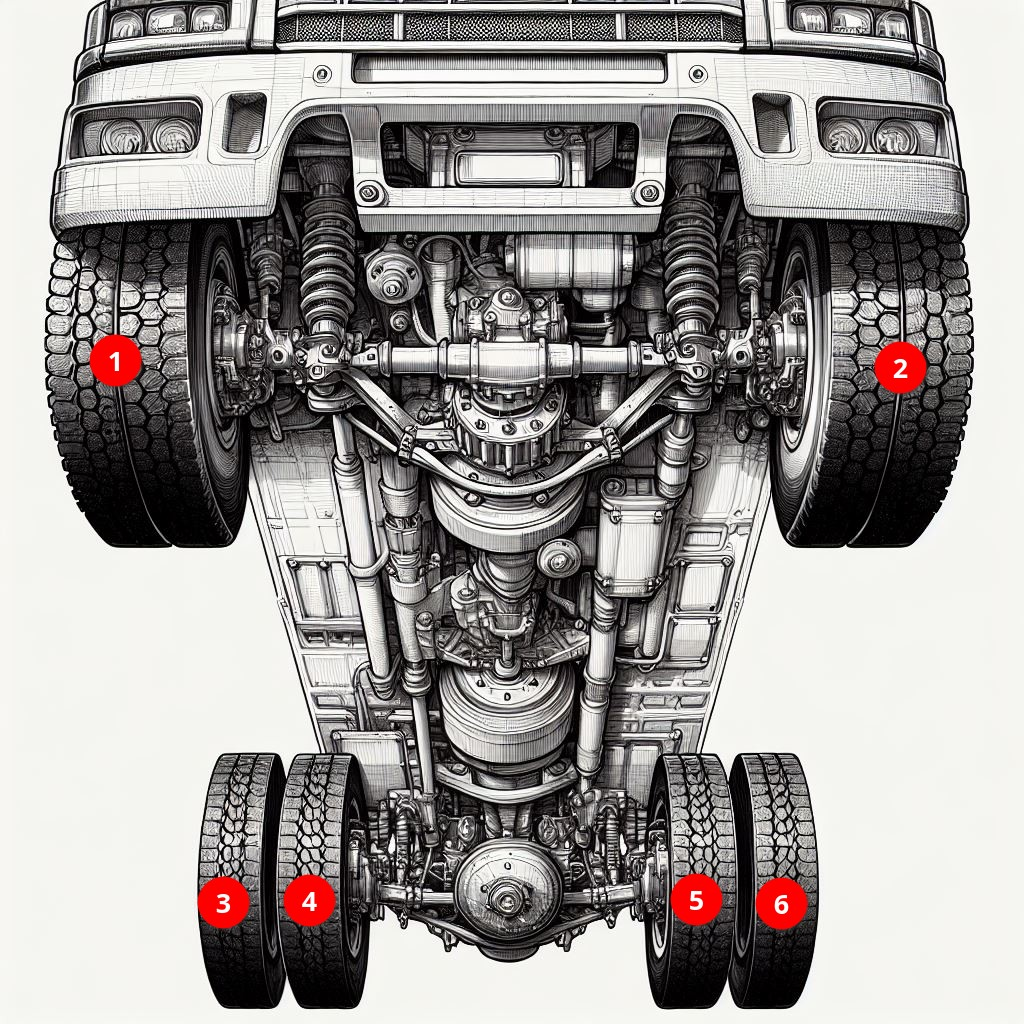
\includegraphics[width=\textwidth]{img/lkw_bottom.jpg}
    \end{column}
    \begin{column}{0.5\textwidth}
      \(R_i\) für Reifen i intakt \\
      \(D_i\) für Reifen i defekt

      Expertenwissen:

      \begin{itemize}
        \item \(D_i \implies \mbox{NICHT}(R_i)\)
        \item FahrzeugOK = R1 UND R2 UND R3 UND R4 UND R5 und R6
        \item NichtFahrbereit = D1 oder D2 oder (D3 und D4) oder (D5 und D6)
      \end{itemize}
    \end{column}
  \end{columns}
\end{frame}

\section{Aussagenlogik}

\begin{frame}{Aussagenlogik}
  \begin{columns}
    \begin{column}{0.65\textwidth}
      \begin{block}{Herkunft}
        Mathematische Grundlagen durch die Boolesche Algebra als Logik-Kalkül (George Boole, 1847)
      \end{block}
      \begin{block}{Anwendungungen}
        \begin{itemize}
          \item \textbf{Aussagenlogik} mit 0 als falsch und 1 als wahr
          \item Mengenlehre
          \item Schaltalgebra mit 0 (Schaltzustand AUS bzw Spannung niedrig) und 1 (Schaltzustand EIN bzw Spannung hoch)
        \end{itemize}

      \end{block}
    \end{column}
    \begin{column}{0.35\textwidth}
      \centering George Boole (1815-1864)
      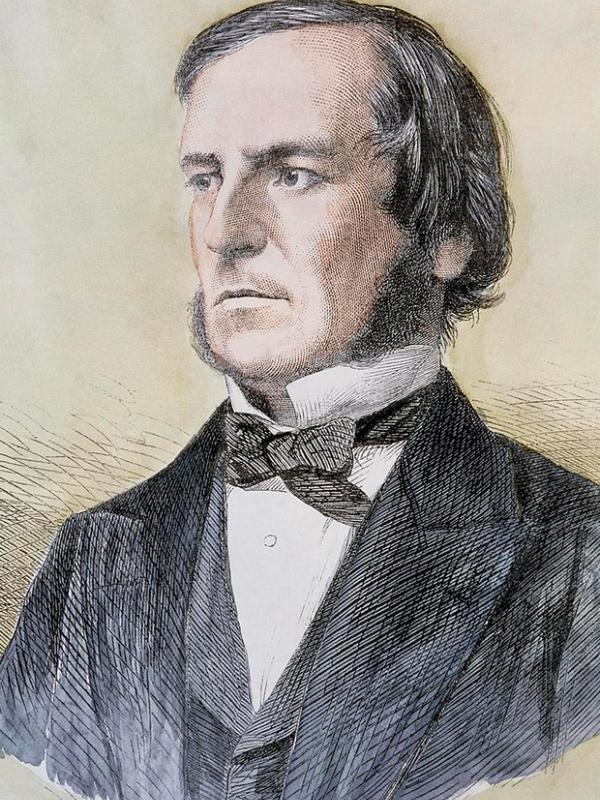
\includegraphics[height=.7\textheight]{img/George_Boole.jpg}
    \end{column}
  \end{columns}
\end{frame}

\begin{frame}{Andere Logiken}
  \begin{columns}
    \begin{column}{0.5\textwidth}
      \begin{exampleblock}{Prädikatenlogik (Erweiterung der Aussagenlogik)}
        \begin{align*}
          \exists x \in \mathbb{N} & : x = \left|x\right| \\
          \forall x \in \mathbb{N} & : x - 1 < x
        \end{align*}
      \end{exampleblock}
      \begin{exampleblock}{Fuzzy Logik}
        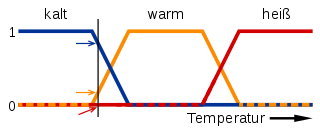
\includegraphics[width=\textwidth]{img/fuzzy_logic.png}
      \end{exampleblock}
    \end{column}
    \begin{column}{0.5\textwidth}
      \begin{exampleblock}{Temporale Logik}
        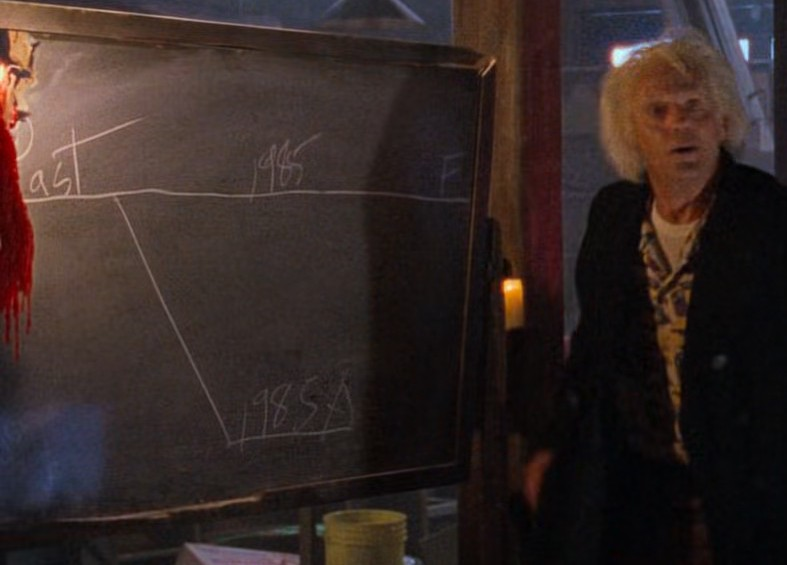
\includegraphics[width=\textwidth]{img/temporal_logic_doc_brown.jpg}
      \end{exampleblock}
    \end{column}
  \end{columns}
\end{frame}

\begin{frame}{Logik-Kalkül (George Boole, 1847)}
  \begin{definition}
    Eine Menge $B$ von Elementen, über der zwei Operationen (\(+\) und (\(\cdot\)) definiert sind, ist genau dann Boolesche Algebra \( B; +, \cdot\) wenn für beliebige Elemente \(a\), \(b\), \(c\) aus \(B\) die folgenden Axiome gelten:
    \begin{itemize}
      \item \textbf{Kommutativgesetz}:
            \begin{itemize}
              \item \(a + b = b + a\)
              \item \(a \cdot b = b \cdot a\)
            \end{itemize}
      \item \textbf{Assoziativgesetz}:
            \begin{itemize}
              \item \(a + (b + c) = (a + b) + c\)
              \item \(a \cdot (b \cdot c) = (a \cdot b) \cdot c\)
            \end{itemize}
      \item \textbf{Distributivgesetz}:
            \(a + (b \cdot c) = (a + b) \cdot (a + c)\)
      \item \textbf{Identitätsgesetz}:
            \(a + 0 = a\) und \(a \cdot 1 = a\)
      \item \textbf{Negationsgesetz}:
            \(a + 1 = 1\) und \(a \cdot 0 = 0\)
      \item \textbf{Idempotenzgesetz}:
            \(a + a = a\) und \(a \cdot a = a\)
            %\item $x^2=x$ und $x+x=x$
    \end{itemize}
  \end{definition}
\end{frame}

\begin{frame}{Aussagenlogik}{Als Boolesche Algebra}
  \begin{definition}
    Die Aussagenlogik ist eine Boolesche Algebra. Es gelten damit die Gesetze der Booleschen Algebra.
  \end{definition}

  \begin{block}{Werte}
    \centering
    \begin{tabular}{ccc}
      \toprule
      \textbf{Wert} & \multicolumn{2}{c}{\textbf{Bezeichnungen}}         \\
      \midrule
      0             & Falsch                                     & False \\
      1             & Wahr                                       & True  \\
      \bottomrule
    \end{tabular}
  \end{block}
\end{frame}

\begin{frame}{Aussagenlogik}{Operationen}
  \begin{block}{Operationen}
    \centering
    \begin{tabular}{lcccc}
      \toprule
      \multicolumn{3}{c}{\textbf{Bezeichnungen}} & \textbf{Symbol} & \textbf{Python-Operator}                                            \\
      \midrule
      Konjunktion                                & \textbf{UND}    & \textbf{AND}             & \(\land\)                          & and \\
      Disjunktion                                & \textbf{ODER}   & \textbf{OR}              & \(\lor\)                           & or  \\
      Negation                                   & \textbf{NICHT}  & \textbf{NOT}             & \(\lnot\) oder \(\overline{WERT}\) & not \\
      \toprule
    \end{tabular}
  \end{block}
\end{frame}

\begin{frame}{Aussagenlogik}{Rechenregeln}
  Defination der Operationen Konjunktion, Disjunktion und Negation über Wahrheitstafeln:
  \begin{columns}[onlytextwidth]
    \begin{column}{0.48\textwidth}
      \begin{block}{Konjunktion}
        \centering\small
        \begin{tabular}{ccc}
          \toprule
          $A$ & $B$ & $A \land B$ \\
          \midrule
          0   & 0   & 0           \\
          0   & 1   & 0           \\
          1   & 0   & 0           \\
          1   & 1   & 1           \\
          \bottomrule
        \end{tabular}
      \end{block}
    \end{column}
    \begin{column}{0.48\textwidth}
      \begin{block}{Disjunktion}
        \centering\small
        \begin{tabular}{ccc}
          \toprule
          $A$ & $B$ & $A \lor B $ \\
          \midrule
          0   & 0   & 0           \\
          0   & 1   & 1           \\
          1   & 0   & 1           \\
          1   & 1   & 1           \\
          \bottomrule
        \end{tabular}
      \end{block}
    \end{column}
  \end{columns}
  \begin{block}{Negation}
    \centering\small
    \begin{tabular}{cc}
      \toprule
      $A$ & $\lnot A$ \\
      \midrule
      0   & 1         \\
      1   & 0         \\
      \bottomrule
    \end{tabular}
  \end{block}
\end{frame}

\begin{frame}{Logik in verschiedenen Systemen}
  \vspace{-1em}
  \begin{columns}
    \begin{column}{0.5\textwidth}
      \begin{block}{Aussagenlogik für Programme}
        \inputminted[firstline=5,lastline=8]{python}{src/logik_example.py}
      \end{block}
    \end{column}
    \begin{column}{0.5\textwidth}
      \begin{block}{Schaltalgerba}
        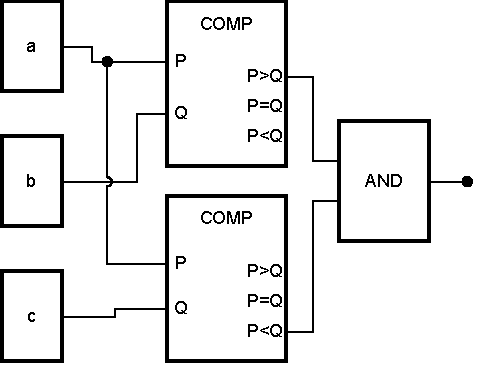
\includegraphics[width=\textwidth]{fig/logik_schaltalgebra.pdf}
      \end{block}
    \end{column}
  \end{columns}
  \vspace{1em}
\end{frame}

\begin{frame}{Bedingungsausdrücke}
  Einzelne Aussagen können Bedingungsausdrücke sein:
  \begin{itemize}
    \item[~] Aussage \texttt{kalt}: \(\mbox{temperatur} < 10\)
    \item[~] Aussage \texttt{zu\_schnell}: \(V > 100\)
  \end{itemize}

  Bedingungsausdrücke werden durch aussagelogische Operationen verknüpft:

  \begin{exampleblock}{Beispiel}
    \begin{align*}
      \lnot \left( zahl < 0 \right) & \land \lnot (zahl > 64) \\
      zahl \geq 0                   & \land zahl \leq 64      \\
      \lnot ( zahl < 0              & \lor zahl > 64 )
    \end{align*}
    \only<2->{Alle drei Ausdrücke sind gleichwertig. zahl ist zwischen 0 und 64.}
  \end{exampleblock}

\end{frame}

% End document
\end{document}
